\documentclass[12pt]{article}

% report, book

%  Русский язык

\usepackage[T2A]{fontenc}
\usepackage[utf8]{inputenc}
\usepackage[english,russian]{babel}

\usepackage{amsmath,amsfonts,amssymb,amsthm,mathtools} 
\usepackage{float}

\usepackage{graphicx}
\usepackage{listings}
\usepackage{hyperref}
\usepackage[table,xcdraw]{xcolor}

\usepackage{wasysym}

\usepackage{geometry} 
\geometry{a4paper,top=2cm,bottom=3cm,left=2cm}

\begin{document}

\begin{titlepage}

\thispagestyle{empty}

\centerline{НИУ ИТМО}
\centerline{Факультет Информационных Технологий и Программирования}
\centerline{Направление "Прикладная Математика и Информатика"}

\vfill

\centerline{\huge{Лабораторная работа 4}}
\centerline{\large{курса ``Методы оптимизации'' }}
\vspace{1cm} 
\centerline{\large{Верблюжий случай}}
\centerline{\large{Сысоев Александр, Зырянова Мария}}
\vfill

\centerline{Санкт-Петербург, 2021}
\clearpage
\end{titlepage}

\section{Постановка задания}

Необходимо разработать и исследовать программы для безусловной минимизации функции многих переменных методом Ньютона и его модификаций.

\begin{enumerate}
	\item Реализовать классический метод Ньютона, с одномерным поиском и с направлением спуска. 
		\begin{enumerate}
			\item Продемонстрировать работу на различных функциях, включая иллюстрации траекторий спуска. Указать количество итераций, необходимых для достижения заданной точности; указывать найденные значения параметров при одномерном поиске.
			\item Исследовать работу на двух функциях с заданным начальным приближением. Сравнить резултаты с минимизацией методом наискорейшего спуска из лабораторной работы 2. Для каждого метода привести иллюстрации траекторий сходимости.
		\end{enumerate}				
	\item Реализовать метод Бройдена-Флетчера-Шено и метод Пауэлла. Работу квазиньютоновских методов сравните с наилучшим методом Ньютона
(по результатам 1.2) на заданных функциях. Провести исследование влияние выбора начального приближения на результат (не менее трех) и оценить скорость сходимости.
	\item Реализовать метод Марквардта двумя вариантами. Результаты работы продемонстрировать на минимизации многомерной функции
Розенброка в сравнении с наилучшим методом Ньютона.
\end{enumerate}

\newpage
\section{Рассматриваемые функции}

\begin{enumerate}
 	\item \[f_1(x) = 50x^2+y^2+20x+20y+239\]
 	Минимум достигается в точке $x_{min} = (-0.2; -10)$, значение минимума -- 137.

 	\item \[ f_2(x) = x_1^4+2x_1^2 x_2-33x_1^2+2x_1 x_2^2-20x_1+x_2^4-19x_2^2-34x_2+389 \]
 	Минимум достигается в
 	\begin{itemize}
 		\item $x_{min} = (-4.562464212637666110367180311; -3.816079691599438559917622764)$;
 		\item $x_{min} = (-3.647700719794428590518679958; 3.694279458811207556710592285)$
 		\item $x_{min} = (3.809451227725493104867729487; 2.488081343580733273436836220)$
 		\item $x_{min} = (4.400713704706601596018130782; -2.366281110792502270229805741)$
 	\end{itemize}
 	Значение минимума во всех случаях 0.

 	\item \[ f_3 = (x-2)^4+(y-3)^4+(z-4)^4\]
 	Минимум достигается в точке $x_{min} = (2; 3; 4)$, значение минимума -- 0.

 	\item \[ f_4 = x_1^2+x_2^2-1.2x_1x_2\]
 	Минимум достигается в точке $x_{min} = (0; 0)$, значение минимума -- 0.

 	\item \[ f_5 = 100 (x_2-x_1^2)^2+(1-x_1)^2\]
 	Минимум достигается в точке $x_{min} = (1; -1)$ и $x_{min} = (1; 1)$, значение минимума -- 0.

 	\item \[ f_6 = (x_1^2+x_2-11)^2+(x_1+x_2^2-7)^2 \]
 	Минимум достигается в
 	\begin{itemize}
 		\item $x_{min} = (3; 2)$;
 		\item $x_{min} = (-3.779310253377746891890765841; -3.283185991286169412266000514)$
 		\item $x_{min} = (-2.805118086952744853053572398; 3.131312518250572965804300723)$
 		\item $x_{min} = (3.584428340330491744944338239; -1.848126526964403553538300209)$
 	\end{itemize}
 	Значение минимума во всех случаях 0.

 	\item \[ f_7 = (x_1+10x_2)^2+5(x_3-x_4)^2+(x_2-2x_3)^4+10(x_1-x_4)^4 \]
 	Минимум достигается в точке $x_{min} = (0; 0; 0; 0)$, значение минимума -- 0.

 	\item \[ f_8 = 100 - \frac{2}{1+\left( \frac{x_1-1}{2} \right) ^2 + \left( \frac{x_2-1}{3} \right) ^2} - \frac{1}{1+\left( \frac{x_1-2}{2} \right) ^2 + \left( \frac{x_2-1}{3} \right) ^2}\]
 	Минимум достигается в точке $x_{min} = (1.291643031517492930227373527; 1)$, значение минимума -- 97.1531028728543166387604846.

 	\item Функция Розенброка:
 	\[ f = \sum_1^{n-1} 100(x_{i+1}-x_i^2)^2+(1-x_i)^2 \]
 	Минимум достигается в точке $x_{i_{min}} = 1$, а $x_{{100}_{min}} = \pm 1$, значение минимума -- 0.0.
\end{enumerate}

\newpage
\section{Метод Ньютона и его модификации}

Метод минимизации Ньютона основывается на следующих рассуждениях.

Пусть дана дважды дифференцируемая целевая функция нескольких переменных $f(x)$, которую необходимо минимизировать. Разложим ее в ряд Тейлора в фиксиованной точке $x$ при произвольном приращении аргумента $\Delta x$:

\[ f(x+\Delta x) = f(x) + \nabla f(x)^T \Delta x + \frac{1}{2} \Delta x^T \nabla^2f(x)\Delta x + o(\lVert x \rVert ^ 2) \]

Пусть $s = \Delta x, \; g(x) = \nabla f(x), \; H(x) = \nabla^2 f(x)$, принебрежем слагаемыми второго порядка малости, получим квадратичную функцию:

\[ q(x) = f(x) + g(x)^Ts + \frac{1}{2} s^T H(x)s \]

Полученная функция достигает минимума при $s: \; H(x)s = -g(x)$, так как необходимое условие минимума -- $\nabla q(x) = 0$:

\[ \nabla q(x) = g(x)+H(x)s \]

Тогда вектор перемещения в точку минимума квадратичной функции

\[ s = -H(x)^{-1} g(x) \]

Метод Ньютона минимизирует положительно определенную квадратичную функцию за один шаг из любой начальной точки $x_0$. Это метод второго порядка, так как используется вычисление гессиана -- вторые частные производные.

\newpage
\subsection{Классический метод Ньютона}

Классический метод Ньютона является итерационным. Обозначая в текущей точке поиска $x_k$ значения градиента $g_k = \nabla f(x_k)$ и матрицы Гессе $H_k = \nabla^2 f(x_k)$ получаются следующие итерационные формулы метода Ньютона:

\[ x_{k+1}=x_k+s_k, \quad H_k s_k = -g_k \]\

Итерационный процесс продолжается по мере выполнения условия прерывания с заданной допустимой погрешностью $\epsilon$: $\lVert x_{k+1} - x_k \rVert > \epsilon$

Вектор $s$ находится за счет решения системы линейных уравнений LU-разложением, реализация которого была подробно рассмотрена в 3 лабораторной работе. Этот вектор задает и направление, и шаг перехода в следующую точку поиска.

Иллюстрация работы:
\begin{enumerate}
	\item Исследование на $f_1$:

	\begin{figure}[H]
    	\centering
    	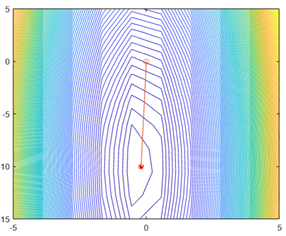
\includegraphics[]{img/f1_1_1.png}
    	\\ Начальное приближение $\left( 0; 0 \right)$
    	\\ Количество итераций: 2
    \end{figure}

	\begin{figure}[H]
    	\centering
    	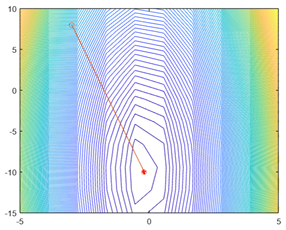
\includegraphics[]{img/f1_1_2.png}
    	\\ Начальное приближение $\left( -3; 8 \right)$
    	\\ Количество итераций: 2
    \end{figure}

	\begin{figure}[H]
    	\centering
    	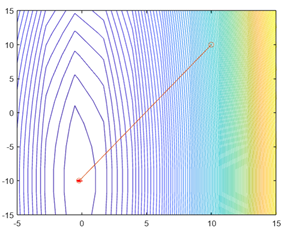
\includegraphics[]{img/f1_1_3.png}
    	\\ Начальное приближение $\left( 10; 10 \right)$
    	\\ Количество итераций: 2
    \end{figure}

	\item Исследование на $f_2$

		\begin{figure}[H]
    	\centering
    	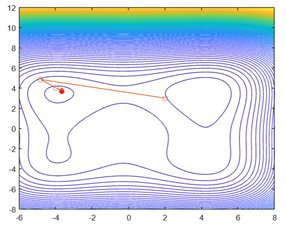
\includegraphics[]{img/f2_1_1.png}
    	\\ Начальное приближение $\left( 2; 3 \right)$
    	\\ Количество итераций: 7
    \end{figure}

	\begin{figure}[H]
    	\centering
    	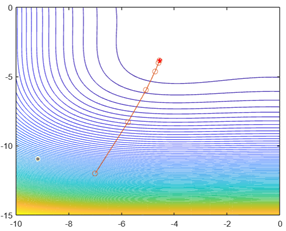
\includegraphics[]{img/f2_1_2.png}
    	\\ Начальное приближение $\left( -7; -12 \right)$
    	\\ Количество итераций: 8
    \end{figure}

	\begin{figure}[H]
    	\centering
    	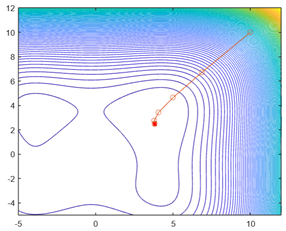
\includegraphics[]{img/f2_1_3.png}
    	\\ Начальное приближение $\left( 10; 10 \right)$
    	\\ Количество итераций: 9
    \end{figure}

	\item Исследование на $f_3$

\begin{table}[H]
\centering
\begin{tabular}{|c|c|c|c|}
\hline
\rowcolor[HTML]{FFF0DB}
{\color[HTML]{333333} \textbf{\begin{tabular}[c]{@{}c@{}}Начальное\\ приближение\end{tabular}}} &
  \textbf{\begin{tabular}[c]{@{}c@{}}Количество\\ итераций\end{tabular}} &
  \textbf{\begin{tabular}[c]{@{}c@{}}Координаты\\ минимума\end{tabular}} &
  \textbf{\begin{tabular}[c]{@{}c@{}}Значение\\ минимума\end{tabular}} \\ \hline
$\left( 1; 2; 3 \right)$ &
  40 &
  \begin{tabular}[c]{@{}c@{}}{[}2.000000102464132, \\ 3.0000001014185793, \\ 4.000000100373027{]}\end{tabular} &
  3.1752354967659026E-28 \\ \hline
$\left( 0; 0; 0 \right)$ &
  43 &
  \begin{tabular}[c]{@{}c@{}}{[}2.000000102851373, \\ 3.000000102644844, \\ 4.000000102438316{]}\end{tabular} &
  3.3302500930352387E-28 \\ \hline
$\left( 10; 10; 10 \right)$ &
  45 &
  \begin{tabular}[c]{@{}c@{}}{[}2.000000091607024, \\ 3.0000000915152336, \\ 4.000000091423443{]}\end{tabular} &
  2.1042463043355587E-28 \\ \hline
\end{tabular}
\end{table}

\end{enumerate}

\newpage
\subsection{Метод Ньютона с одномерным поиском}

Формулы метода Ньютона основаны на аппроксимации функции квадратичной функцией в малой окрестности текущей точки поиска и могут приводить к возрастанию значений функции. Для улучшения применяется одномерная минимизация функции в направлении поиска $s$.

На каждой итерации такого модифицированного метода Ньютона из точки $x_k$ выполняется одномерный поиск в направлении метода Ньютона $d_k = s_k$:

\[ \lambda_k = arg min f(x_k+\lambda d_k) \]

Таким образом, итерационный процесс дополняется следующими формулами:

\[ H_k d_k = -g_k, \quad r = arg min f(x_k+\lambda d_k), \quad s = r \cdot d \]

Метод Ньютона с одномерным поиском надежнее исходного метода Ньютона за счет обеспечения убывания значений целевой функции. Однако его эффективность существенно зависит от того, является ли направление поиска направлением спуска.

Иллюстрация работы:
\begin{enumerate}
	\item Исследование на $f_1$:

	\begin{figure}[H]
    	\centering
    	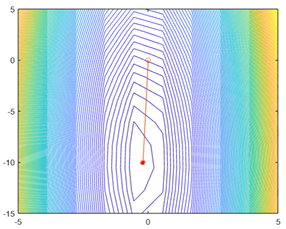
\includegraphics[]{img/f1_2_1.png}
    	\\ Начальное приближение $\left( 0; 0 \right)$
    	\\ Количество итераций: 2
    \end{figure}

	\begin{figure}[H]
    	\centering
    	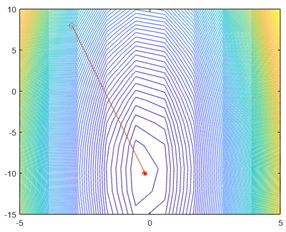
\includegraphics[]{img/f1_2_2.png}
    	\\ Начальное приближение $\left( -3; 8 \right)$
    	\\ Количество итераций: 2
    \end{figure}

	\begin{figure}[H]
    	\centering
    	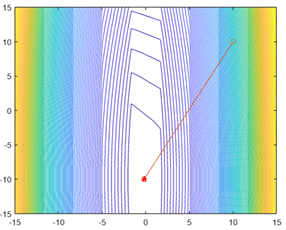
\includegraphics[]{img/f1_2_3.png}
    	\\ Начальное приближение $\left( 10; 10 \right)$
    	\\ Количество итераций: 2
    \end{figure}

	\item Исследование на $f_2$

		\begin{figure}[H]
    	\centering
    	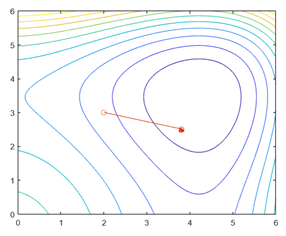
\includegraphics[]{img/f2_2_1.png}
    	\\ Начальное приближение $\left( 2; 3 \right)$
    	\\ Количество итераций: 7
    \end{figure}

	\begin{figure}[H]
    	\centering
    	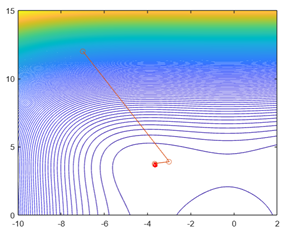
\includegraphics[]{img/f2_2_2.png}
    	\\ Начальное приближение $\left( -7; -12 \right)$
    	\\ Количество итераций: 8
    \end{figure}

	\begin{figure}[H]
    	\centering
    	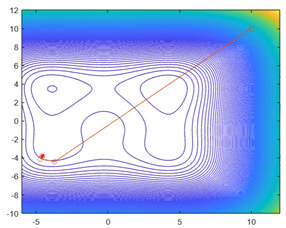
\includegraphics[]{img/f2_2_3.png}
    	\\ Начальное приближение $\left( 10; 10 \right)$
    	\\ Количество итераций: 9
    \end{figure}

	\item Исследование на $f_3$

\begin{table}[H]
\centering
\begin{tabular}{|c|c|c|c|}
\hline
\rowcolor[HTML]{FFF0DB}
{\color[HTML]{333333} \textbf{\begin{tabular}[c]{@{}c@{}}Начальное\\ приближение\end{tabular}}} &
  \textbf{\begin{tabular}[c]{@{}c@{}}Количество\\ итераций\end{tabular}} &
  \textbf{\begin{tabular}[c]{@{}c@{}}Координаты\\ минимума\end{tabular}} &
  \textbf{\begin{tabular}[c]{@{}c@{}}Значение\\ минимума\end{tabular}} \\ \hline
$\left( 1; 2; 3 \right)$ &
  2 &
  \begin{tabular}[c]{@{}c@{}}{[}2.0, \\ 3.0, \\ 4.0{]}\end{tabular} &
  3.1859327586943765E-28 \\ \hline
$\left( 0; 0; 0 \right)$ &
  2 &
  \begin{tabular}[c]{@{}c@{}}{[}1.9999999999999998, \\ 3.0, \\ 3.9999999999999996{]}\end{tabular} &
  3.1029304856675849E-28 \\ \hline
$\left( 10; 10; 10 \right)$ &
  2 &
  \begin{tabular}[c]{@{}c@{}}{[}2.0, \\ 3.0, \\ 4.0{]}\end{tabular} &
  3.0004873436292834E-28 \\ \hline
\end{tabular}
\end{table}


\end{enumerate}

\newpage
\subsection{Метод Ньютона с направлением спуска}

Гарантией убывания значения функции является нахождение такого направления одномерного поиска, которое будет и направлением спуска. Метод Ньютона приводит к ошибочному направлению в точке максимума и в седловых точках.

$s_k$ -- направление спуска, если скалярное произведение вектора направления из точки $x_k$ и вектора градиента в этой точке отрицательно (то есть между ними образуется тупой угол). Если же угол острый, то $s_k$ не является направлением убывания, следовательно, разумнее использовать направление антиградиента, так как оно гарантирует убывание функции.

Таким образом, направление спуска задается следующим образом:

\[ H_k s_k = -g_k \]
\[ d_k =
	\begin{cases}
		s_k, \quad s_k^t g_k < 0 \\
		-g_k, \quad s_k^t g_k \geq 0
	\end{cases}
\]

Накопленный опыт показал, что первую итерацию разумнее проводить в направлении антиградиента с использованием одномерного поиска. Тогда на первом шаге $d_0 = -g_0, \; r_0 = arg min f(x_0+\lambda d_0), \; s_0 = r_0 \cdot d_0, \; x_1 = x_0 + s_0$. Далее выполняется итерационный процесс, пока $\lVert s_k \rVert > \epsilon$:

\begin{enumerate}
 	\item $Hs = -g$
 	\item Если $s^T \cdot g < 0$, то $d = s$, иначе $d = -g$
 	\item $r = arg min f(x+\lambda d), \; s = rd$
 	\item $x = x + s$
\end{enumerate}

Иллюстрация работы:
\begin{enumerate}
	\item Исследование на $f_1$:

	\begin{figure}[H]
    	\centering
    	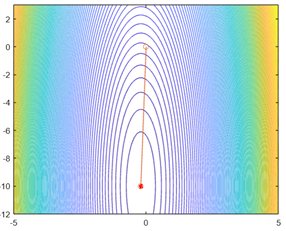
\includegraphics[]{img/f1_3_1.png}
    	\\ Начальное приближение $\left( 0; 0 \right)$
    	\\ Количество итераций: 2
    \end{figure}

	\begin{figure}[H]
    	\centering
    	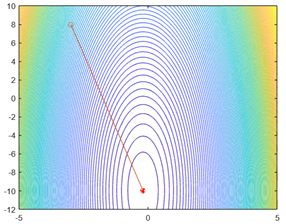
\includegraphics[]{img/f1_3_2.png}
    	\\ Начальное приближение $\left( -3; 8 \right)$
    	\\ Количество итераций: 2
    \end{figure}

	\begin{figure}[H]
    	\centering
    	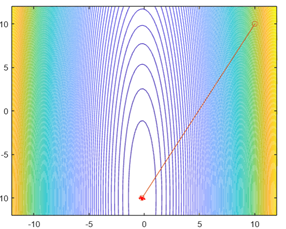
\includegraphics[]{img/f1_3_3.png}
    	\\ Начальное приближение $\left( 10; 10 \right)$
    	\\ Количество итераций: 2
    \end{figure}

	\item Исследование на $f_2$

		\begin{figure}[H]
    	\centering
    	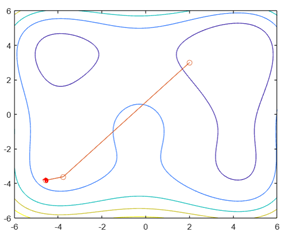
\includegraphics[]{img/f2_3_1.png}
    	\\ Начальное приближение $\left( 2; 3 \right)$
    	\\ Количество итераций: 7
    \end{figure}

	\begin{figure}[H]
    	\centering
    	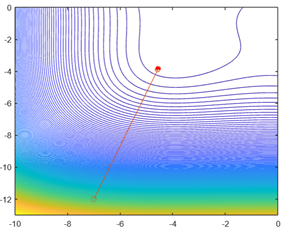
\includegraphics[]{img/f2_3_2.png}
    	\\ Начальное приближение $\left( -7; -12 \right)$
    	\\ Количество итераций: 8
    \end{figure}

	\begin{figure}[H]
    	\centering
    	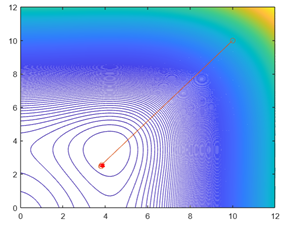
\includegraphics[]{img/f2_3_3.png}
    	\\ Начальное приближение $\left( 10; 10 \right)$
    	\\ Количество итераций: 9
    \end{figure}

	\item Исследование на $f_3$

\begin{table}[H]
\centering
\begin{tabular}{|c|c|c|c|}
\hline
\rowcolor[HTML]{FFF0DB}
{\color[HTML]{333333} \textbf{\begin{tabular}[c]{@{}c@{}}Начальное\\ приближение\end{tabular}}} &
  \textbf{\begin{tabular}[c]{@{}c@{}}Количество\\ итераций\end{tabular}} &
  \textbf{\begin{tabular}[c]{@{}c@{}}Координаты\\ минимума\end{tabular}} &
  \textbf{\begin{tabular}[c]{@{}c@{}}Значение\\ минимума\end{tabular}} \\ \hline
$\left( 1; 2; 3 \right)$ &
  1 &
  \begin{tabular}[c]{@{}c@{}}{[}2.0000000000000004, \\ 3.0000000000000004, \\ 4.0{]}\end{tabular} &
  3.1752354967659026E-28 \\ \hline
$\left( 0; 0; 0 \right)$ &
  2 &
  \begin{tabular}[c]{@{}c@{}}{[}2.0, \\ 3.0, \\ 4.0{]}\end{tabular} &
  3.3302500930352387E-28 \\ \hline
$\left( 10; 10; 10 \right)$ &
  2 &
  \begin{tabular}[c]{@{}c@{}}{[}2.0, \\ 3.0, \\ 4.0{]}\end{tabular} &
  2.1042463043355587E-28 \\ \hline
\end{tabular}
\end{table}

\end{enumerate}

\newpage
\subsection{Сравнение методов Ньютона}

Сравнение производится между тремя методами Ньютона и методом наискорейшего спуска, реализованного в лабораторной работе №2.

\begin{enumerate}
	\item Исследование на $f_4$

	\begin{figure}[H]
	\begin{minipage}{.5\textwidth}
    	\centering
    	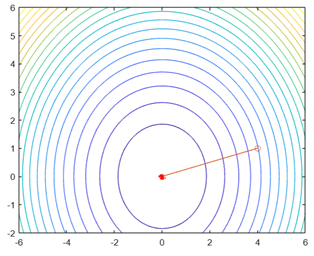
\includegraphics[scale=0.75]{img/f3_1.png}
		\\ Классический метод Ньютона
		\\ Количество итераций: 2
	\end{minipage}
    \begin{minipage}{.5\textwidth}
    \centering
    	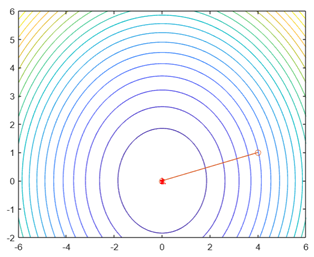
\includegraphics[scale=0.75]{img/f3_2.png}
    	\\ С одномерным поиском
    	\\ Количество итераций: 2
    \end{minipage}
    \end{figure}

	\begin{figure}[H]
	\begin{minipage}{.5\textwidth}
    	\centering
    	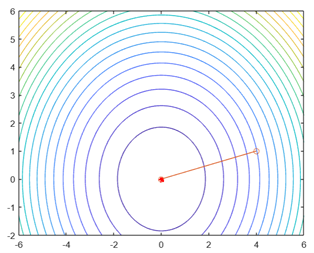
\includegraphics[scale=0.75]{img/f3_3.png}
		\\ С направлением спуска
		\\ Количество итераций: 2
	\end{minipage}
    \begin{minipage}{.5\textwidth}
    \centering
    	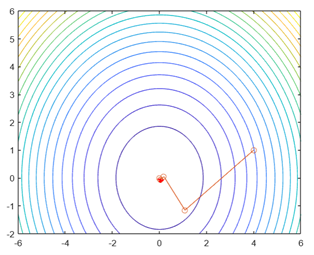
\includegraphics[scale=0.75]{img/f3_4.png}
    	\\ Метод наискорейшего спуска
    	\\ Количество итераций: 15
    \end{minipage}
    \end{figure}

    \begin{figure}[H]
    	\centering
    	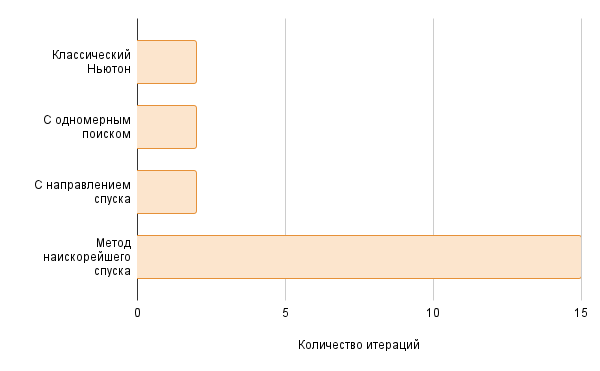
\includegraphics[scale=0.6]{img/chart.png}
    \end{figure}

	\item Исследование на $f_5$

	\begin{figure}[H]
	\begin{minipage}{.5\textwidth}
    	\centering
    	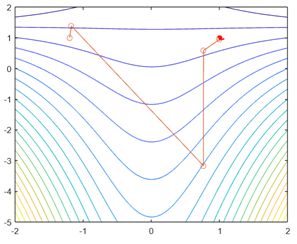
\includegraphics[scale=0.75]{img/f4_1.png}
		\\ Классический метод Ньютона
		\\ Количество итераций: 7
	\end{minipage}
    \begin{minipage}{.5\textwidth}
    \centering
    	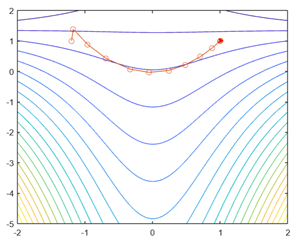
\includegraphics[scale=0.75]{img/f4_2.png}
    	\\ С одномерным поиском
    	\\ Количество итераций: 14
    \end{minipage}
    \end{figure}

	\begin{figure}[H]
	\begin{minipage}{.5\textwidth}
    	\centering
    	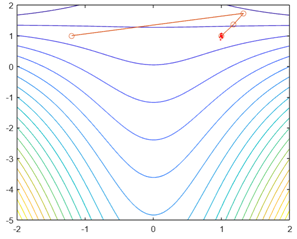
\includegraphics[scale=0.75]{img/f4_3.png}
		\\ С направлением спуска
		\\ Количество итераций: 6
	\end{minipage}
    \begin{minipage}{.5\textwidth}
    \centering
    	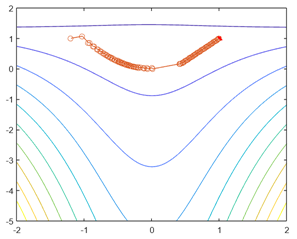
\includegraphics[scale=0.75]{img/f4_4.png}
    	\\ Метод наискорейшего спуска
    	\\ Количество итераций: 90
    \end{minipage}
    \end{figure}

    \begin{figure}[H]
    	\centering
    	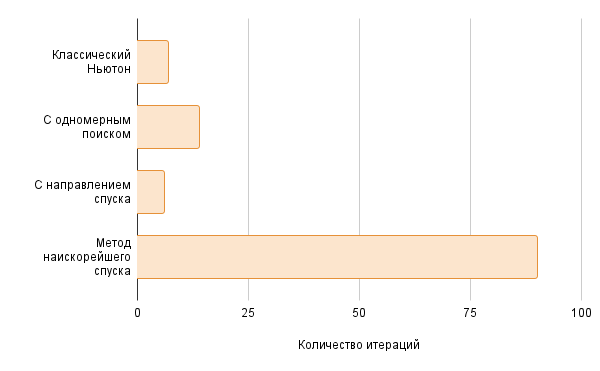
\includegraphics[scale=0.6]{img/chart_1.png}
    \end{figure}
\end{enumerate}

\newpage
\section{Квазиньютоновские методы}

Квазиньютоновские методы основываются на методе Ньютона с одномерным поиском. В методах Ньютона требуется вычисление гессиана, что при больших размерностях пространства требует больших затрат машинного времени, поэтому разумно аппроксимировать матрицу Гессе или обратную к ней с использованием значений градиента. В итоге, получается метод первого порядка.

Гессиан -- симметрическая матрица, поэтому и обратная к ней $G(x)$ тоже симметрическая. Зададим ее начальное приближение в виде некоторой симметрической положительно определенной матрицы $G_0$. Такое задание обеспечивает соответствующее направление одномерного поиска $d_0=-G_0g_0$ из начальной точки $x_0$ как направление спуска. Следующая точка ищется так:

\[ x_1 = x_0+\lambda_0 d_0, \; \text{где} \; \lambda_0=arg min f(x_0+\lambda d_0) \]

В последующих итерациях построение аппроксимирующей матрицы основано на свойстве квадратичной функции:

\[ g_{k+1}-g_k = H(x_{k+1}-x_k) \]

Пусть $p_k=g_{k+1}-g_k, \; s_k = x_{k+1}-x_k$, тогда $Gp_k=s_k$. Если известна аппроксимация для $G$, то следующее ее приближение в точке $x_{k+1}$ должно удовлетворять уравнению

\[ G_{k+1}p_k = s_k \]

Но найти такую матрицу невозможно, так как количество неизвестных в силу симметричности $G$ превышает количество уравнений $n$. Поэтому используется дополнительное условие -- уравнение коррекции:

\[ G_{k+1} = G_k + \Delta G_k \]

Различные квазиньютоновские методы отличаются между собой формулами для поправки $\Delta G_k$.

\subsection{Метод Бройдена-Флетчера-Шено}

В данном методе аппроксимируется сама матрица Гессе по принципу: $H_{k+1}s_k = p_k$. Для нее поправка имеет вид:

\[ \frac{p_k p_k^T}{p_k^t s_k} - \frac{H_k s_k (H_k s_k)^T}{(H_k s_k)^T s_k} \]

Поскольку аппроксимируется гессиан, а не обратная матрица, направление поиска ищется путем решения СЛАУ: $H_k d_k = -g_k$.

\subsection{Метод Пауэлла}

\[ \Delta G_k = - \frac{u \cdot u^T}{\left(u^T, p \right)} \]

где $u_k = s_k - G_kp, \; p = \nabla f(x_{k+1}) - \nabla f(x_{k})$.

Направление одномерного поиска $d_k = -Gg_k$.

\subsection{Сравнение методов}

\begin{enumerate}
	\item Исследование на $f_5$
	\begin{enumerate}

	\item Метод Бройдена-Флетчера-Шено
	\begin{figure}[H]
	\begin{minipage}{.5\textwidth}
    	\centering
    	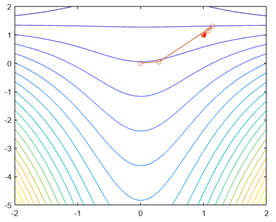
\includegraphics[]{img/f5_1_1.png}
    	\\ Начальное приближение $\left( 0; 0 \right)$
    	\\ Количество итераций: 11
	\end{minipage}
	\begin{minipage}{.5\textwidth}
    	\centering
    	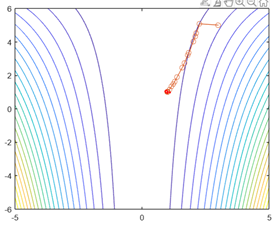
\includegraphics[]{img/f5_1_2.png}
    	\\ Начальное приближение $\left( 3; 5 \right)$
    	\\ Количество итераций: 20
	\end{minipage}
    \end{figure}

	\begin{figure}[H]
    	\centering
    	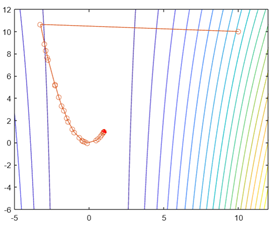
\includegraphics[]{img/f5_1_3.png}
    	\\ Начальное приближение $\left( 10; 10 \right)$
    	\\ Количество итераций: 31
    \end{figure}

	\item Метод Пауэлла
	\begin{figure}[H]
	\begin{minipage}{.5\textwidth}
    	\centering
    	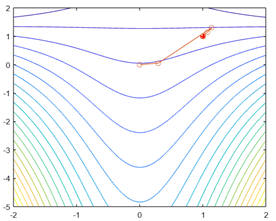
\includegraphics[]{img/f5_2_1.png}
    	\\ Начальное приближение $\left( 0; 0 \right)$
    	\\ Количество итераций: 11
	\end{minipage}
	\begin{minipage}{.5\textwidth}
    	\centering
    	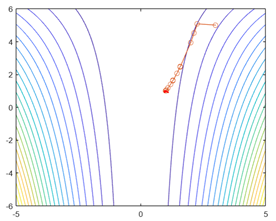
\includegraphics[]{img/f5_2_2.png}
    	\\ Начальное приближение $\left( 3; 5 \right)$
    	\\ Количество итераций: 19
	\end{minipage}
    \end{figure}

	\begin{figure}[H]
    	\centering
    	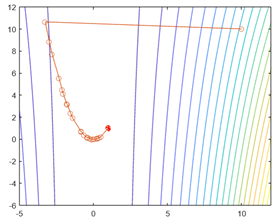
\includegraphics[]{img/f5_2_3.png}
    	\\ Начальное приближение $\left( 10; 10 \right)$
    	\\ Количество итераций: 31
    \end{figure}

	\item Метод Ньютона с направлением спуска

	\begin{figure}[H]
	\begin{minipage}{.5\textwidth}
    	\centering
    	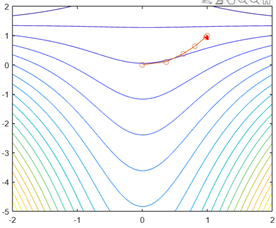
\includegraphics[]{img/f5_3_1.png}
    	\\ Начальное приближение $\left( 0; 0 \right)$
    	\\ Количество итераций: 8
	\end{minipage}
	\begin{minipage}{.5\textwidth}
    	\centering
    	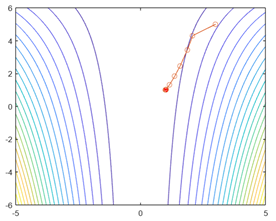
\includegraphics[]{img/f5_3_2.png}
    	\\ Начальное приближение $\left( 3; 5 \right)$
    	\\ Количество итераций: 10
	\end{minipage}
    \end{figure}

	\begin{figure}[H]
    	\centering
    	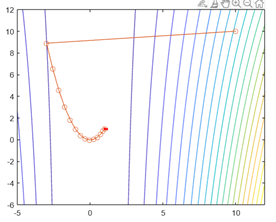
\includegraphics[]{img/f5_3_3.png}
    	\\ Начальное приближение $\left( 10; 10 \right)$
    	\\ Количество итераций: 18
    \end{figure}

	\end{enumerate}

	\item Исследование на $f_6$
	\begin{enumerate}

	\item Метод Бройдена-Флетчера-Шено
	\begin{figure}[H]
	\begin{minipage}{.5\textwidth}
    	\centering
    	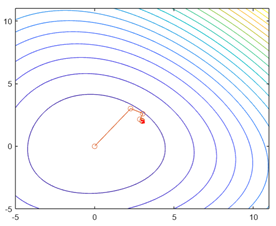
\includegraphics[]{img/f6_1_1.png}
    	\\ Начальное приближение $\left( 0; 0 \right)$
    	\\ Количество итераций: 9
	\end{minipage}
	\begin{minipage}{.5\textwidth}
    	\centering
    	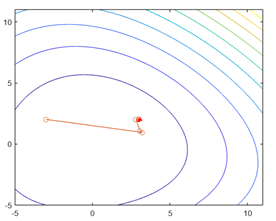
\includegraphics[]{img/f6_1_2.png}
    	\\ Начальное приближение $\left( -3; 2 \right)$
    	\\ Количество итераций: 11
	\end{minipage}
    \end{figure}

	\begin{figure}[H]
    	\centering
    	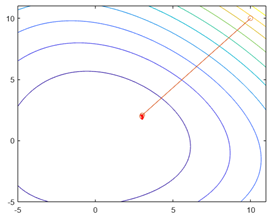
\includegraphics[]{img/f6_1_3.png}
    	\\ Начальное приближение $\left( 10; 10 \right)$
    	\\ Количество итераций: 7
    \end{figure}

	\item Метод Пауэлла
	\begin{figure}[H]
	\begin{minipage}{.5\textwidth}
    	\centering
    	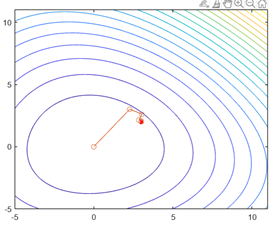
\includegraphics[]{img/f6_2_1.png}
    	\\ Начальное приближение $\left( 0; 0 \right)$
    	\\ Количество итераций: 9
	\end{minipage}
	\begin{minipage}{.5\textwidth}
    	\centering
    	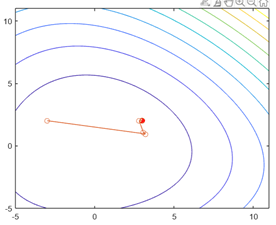
\includegraphics[]{img/f6_2_2.png}
    	\\ Начальное приближение $\left( -3; 2 \right)$
    	\\ Количество итераций: 9
	\end{minipage}
    \end{figure}

	\begin{figure}[H]
    	\centering
    	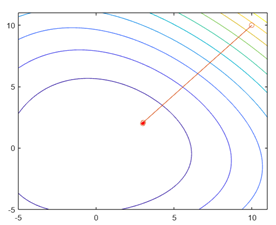
\includegraphics[]{img/f6_2_3.png}
    	\\ Начальное приближение $\left( 10; 10 \right)$
    	\\ Количество итераций: 7
    \end{figure}

	\item Метод Ньютона с направлением спуска

	\begin{figure}[H]
	\begin{minipage}{.5\textwidth}
    	\centering
    	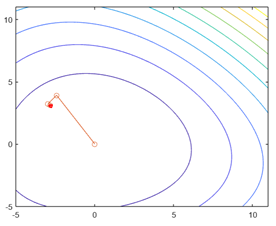
\includegraphics[]{img/f6_3_1.png}
    	\\ Начальное приближение $\left( 0; 0 \right)$
    	\\ Количество итераций: 8
	\end{minipage}
	\begin{minipage}{.5\textwidth}
    	\centering
    	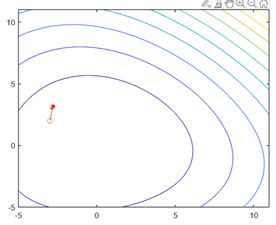
\includegraphics[]{img/f6_3_2.png}
    	\\ Начальное приближение $\left( -3; 2 \right)$
    	\\ Количество итераций: 8
	\end{minipage}
    \end{figure}

	\begin{figure}[H]
    	\centering
    	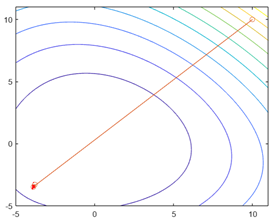
\includegraphics[]{img/f6_3_3.png}
    	\\ Начальное приближение $\left( 10; 10 \right)$
    	\\ Количество итераций: 6
    \end{figure}

	\end{enumerate}

	\item Исследование на $f_7$

	\begin{table}[H]
	\centering
\begin{tabular}{|c|c|c|c|}
\hline
\rowcolor[HTML]{FFF0DB}
{\color[HTML]{333333} \textbf{}} & \textbf{Метод БФШ} & \textbf{Метод Пауэлла} & \textbf{Метод Ньютона} \\ \hline
$\left( 10; 10; 10; 10 \right)$ & 24 & 26 & 18 \\ \hline
$\left( -3; 7; 2; 5 \right)$    & 33 & 31 & 28 \\ \hline
$\left( 4; 6; -8; 4 \right)$    & 18 & 18 & 25 \\ \hline
\end{tabular}
\end{table}

	\item Исследование на $f_8$
	\begin{enumerate}

	\item Метод Бройдена-Флетчера-Шено
	\begin{figure}[H]
	\begin{minipage}{.5\textwidth}
    	\centering
    	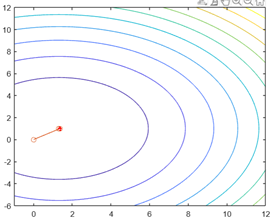
\includegraphics[]{img/f8_1_1.png}
    	\\ Начальное приближение $\left( 0; 0 \right)$
    	\\ Количество итераций: 35
	\end{minipage}
	\begin{minipage}{.5\textwidth}
    	\centering
    	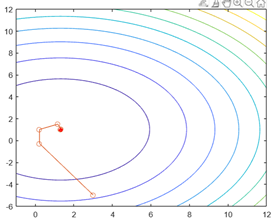
\includegraphics[]{img/f8_1_2.png}
    	\\ Начальное приближение $\left( 3; -5 \right)$
    	\\ Количество итераций: 28
	\end{minipage}
    \end{figure}

	\begin{figure}[H]
    	\centering
    	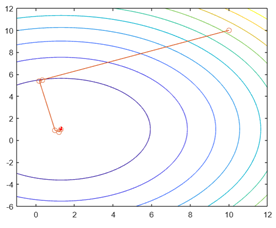
\includegraphics[]{img/f8_1_3.png}
    	\\ Начальное приближение $\left( 10; 10 \right)$
    	\\ Количество итераций: 8
    \end{figure}

	\item Метод Пауэлла
	\begin{figure}[H]
	\begin{minipage}{.5\textwidth}
    	\centering
    	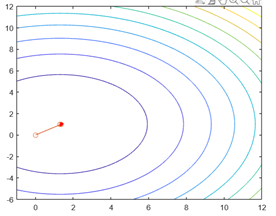
\includegraphics[]{img/f8_2_1.png}
    	\\ Начальное приближение $\left( 0; 0 \right)$
    	\\ Количество итераций: 30
	\end{minipage}
	\begin{minipage}{.5\textwidth}
    	\centering
    	\includegraphics[]{img/f8_2_2.png}
    	\\ Начальное приближение $\left( 3; -5 \right)$
    	\\ Количество итераций: 49
	\end{minipage}
    \end{figure}

	\begin{figure}[H]
    	\centering
    	\includegraphics[]{img/f8_2_3.png}
    	\\ Начальное приближение $\left( 10; 10 \right)$
    	\\ Количество итераций: 10
    \end{figure}

	\item Метод Ньютона с направлением спуска

	\begin{figure}[H]
	\begin{minipage}{.5\textwidth}
    	\centering
    	\includegraphics[]{img/f8_3_1.png}
    	\\ Начальное приближение $\left( 0; 0 \right)$
    	\\ Количество итераций: 29
	\end{minipage}
	\begin{minipage}{.5\textwidth}
    	\centering
    	\includegraphics[]{img/f8_3_2.png}
    	\\ Начальное приближение $\left( 3; -5 \right)$
    	\\ Количество итераций: 37
	\end{minipage}
    \end{figure}

	\begin{figure}[H]
    	\centering
    	\includegraphics[]{img/f8_3_3.png}
    	\\ Начальное приближение $\left( 10; 10 \right)$
    	\\ Количество итераций: 52
    \end{figure}

	\end{enumerate}
\end{enumerate}

\newpage
\section{Метод Марквардта}

Этот метод является комбинацией методов наискорейшего спуска и метода Ньютона. Движение в направлении антиградиента из начальной точки поиска обычно приводит к существенному уменьшению целевой функции. С другой стороны, направления эффективного поиска в окрестности точки минимума определяются по методу Ньютона.

Этот метод и его модификация характеризуются относительной простотой, свойством убывания $f(x)$ при переходе от итерации к итерации, высокой скоростью сходимости в окрестности $x^*$ и отсутствием процедуры одномерного поиска.

\subsection{Обычный метод Марквардта}

В данном методе используется следующая идея ($\alpha$ -- скалярный параметр, $E$ -- единичная матрица):

\[ \left( H(x) + \alpha E \right) s = -g(x) \]

\begin{enumerate}
	\item При большом значении $\alpha$ матрицей $H$ можно пренебречь, тогда получается уравнение $\alpha Es = -g(x)$, и в этом случае направление вектора $s$ совпадает с антиградиентом (направление наискорейшего спуска).
	\item При $\alpha \rightarrow 0$ можно пренебречь $\alpha E$, тогда $s$ -- шаг метода Ньютона.
\end{enumerate}

Таким образом, выбрав начальное значение $\alpha_0$ достаточно большим, а затем уменьшая его, сначала будут выполняться шаги наискорейшего спуска, а на конечных этапах -- метода Ньютона.

В общем виде:

\[ x_{k+1} = x_k + s_k, \; \left( H_k + \alpha_k E \right) s_k = -g_k, \; \alpha_k = \alpha{k-1} \beta \].

Но если значение функции в новой точке больше, чем в предыдушей, то требуется корректировка $\alpha := \frac{\alpha}{\beta}$.

\subsection{Метод Марквардта с применением разложения Холецкого}

Можно начинать с $\alpha_0 = 0$, тогда на каждой итерации должно выполняться условие на $ H+\alpha E$ -- она должна быть положительно определенная. Если это условие не выполняется, то перевыбирается $\alpha = max \left( 1, 2\alpha \right)$.

Условие положительно определенной формы проверяется с помощью разложения Холецкого: $H+\alpha I = LL^T$, где $L$ -- нижнетреугольная матрица. Тогда если такое разложение возможно, то она положительно определена.

Сложность метода в таком случае будет складываться из числа запусков алгоритма Холецкого. Его сложность -- $O(n^3)$

\subsection{Исследование на функции Розенброка}

\begin{table}[H]
\begin{tabular}{|c|c|c|c|}
\hline
\rowcolor[HTML]{FFF0DB}
{\color[HTML]{333333} \textbf{}} &
  \textbf{\begin{tabular}[c]{@{}c@{}}С направлением\\ спуска\end{tabular}} &
  \textbf{Метод Марквардта} &
  \textbf{\begin{tabular}[c]{@{}c@{}}С разложением\\ Холецкого\end{tabular}} \\ \hline
Количество итераций                                                                & 7   & 4881 & 143 \\ \hline
\begin{tabular}[c]{@{}c@{}}Количество подсчетов\\ значения функции\end{tabular}    & 287 & 4882 & 0   \\ \hline
\begin{tabular}[c]{@{}c@{}}Уоличество подстчетов\\ значения градиента\end{tabular} & 7   & 153  & 143 \\ \hline
\begin{tabular}[c]{@{}c@{}}Уоличество подстчетов\\ значения гессиана\end{tabular}  & 6   & 153  & 143 \\ \hline
\end{tabular}
\end{table}

Кликабельно:

\begin{itemize}

\item \href{https://github.com/Mr3zee/Newton-Optimization/blob/docs/docs/marquardt_alpha.txt}{Значения параметра $\alpha$ для обычного метода Марквардта}.

\item \href{https://github.com/Mr3zee/Newton-Optimization/blob/docs/docs/marquardt_cholesky_alpha.txt}{Значения параметра $\alpha$ для метода Марквардта с разложением Холецкого}.

\end{itemize}




\newpage
\section{Выводы}

Основной недостаток методов Ньютона -- использование матрицы вторых частных производных, требующее дополнительных вычислений.

Классический метод Ньютона может расходиться для функции общего вида, возможно возрастание функции от итерации к итерации. Метод Ньютона с одномерным поиском частично устраняет этот недостаток классического метода. Однако его эффективность существенно зависит от того, является ли направление поиска направлением спуска.

Самый надежный из них и требующий наименьшего количества итераций метод -- метод Ньютона с направлением спуска. Однако, все три метода ведут себя лучше реализованного ранее метода наискорейшего спуска.

Недостаток метода Пауэлла -- возможность обращения в нуль знаменателя прибавки. Это происходит в случае, когда $s_k$ совпадает с направлением предыдущей итерации, и матрица $G_{k+1}$ становится вырожденной или неопределенной. Методы Бройдена-Флетчера-Шено и Пауэлла примерно равны между собой и различаются количеством внутренних вычислений. Хоть и метод Ньютона с направлением спуска работает за меньшее число итераций, эти два метода требуют меньшее число сложных вычислений (как, например, решение СЛАУ).

Метод Марквардта позволяет устранить недостатки метода Ньютона -- невозможность корректировки длины шага и возможно плохую обсуловленность СЛАУ. С применением разложения Холецкого требуется меньшее количество итераций, чтобы найти точку минимума.

Реализация: \href{https://github.com/Mr3zee/Newton-Optimization}{GitHub}.

\end{document}